\chapter{Introduction to the nonperturbative renormalization techniques}

At the so-called Lifshitz critical point, three phases intersect. This is rather unusual, so we expect the physics of the vicinity of this point to be of special interest. To investigate it, we would like to compute the critical exponents associated to this transition point. To this end, we used the powerful machinery of the renormalization group, and more precisely of one particular implementation of the renormalization ideas: the nonpertubative renormalization group.

In this chapter we propose first a very general introduction to the ideas and concepts of renormalization. Then we focus on the nonperturbative renormalization group techniques.

\section{Introduction to the renormalization group}

\subsection{The renormalization procedure}

The idea of renormalization is to reduce the number of degrees of freedom of a given many-body correlated system.
To achieve that, an \textit{effective Hamiltonian at length scale $S$} is built. 
To be more precise, let us imagine that we want to describe a magnetic crystal. The microscopic Hamiltonian will be in general a discrete sum of local observables $O_\alpha$, depending on the value of the local magnetization at site $i$, $\phi(i)$:
\begin{equation}
H[\phi] = \sum_i \sum_\alpha \kappa_\alpha O_\alpha[\phi(i), \nabla \phi(i), ...]
\end{equation}
where $\kappa_\alpha$ is the coupling constant associated to the observable $O_\alpha$. 
This Hamiltonian describe the system at the microscopic scale $S=1$. Now, if we want to describe it at a scale $S \geq 1$, surely we are no longer interested in knowing the fluctuations of the field over regions of size smaller than $a S$\footnote{Experimentally, we can imagine that looking at the system at scale $S$ means probing it with devices having a spatial resolution of $a S$. Any measurement operation with such devices can be described mathematically by the convolution of an observable by an error function having a spatial support of diameter $a S$. This operation is roughly equivalent to averaging the observables (and therefore the field) on blocks of size $a S$.}, where $a$ is the typical distance between two sites. All we need is thus the average over regions of size $a S$ of the field:
\begin{equation}
\tilde{\phi}(b) = \frac{1}{(aS)^d} \sum_{i \in B(b)} \phi(i)
\end{equation}
where $d$ is the dimension of space, and $B(b)$ is the set of sites $i$ belonging to the block $b$.

Schematically what we do is group spins by blocks of size $a S$ (fig. \eqref{renorm_1}), and average over these blocks.

\begin{figure}[htp]
\centering
\begin{subfigure}{.25\textwidth}
	\centering
	
\includegraphics[width=.9\linewidth]{img/chap2/renorm_step0.pdf}
	\caption{The initial lattice.}
	\label{renorm_0}
	\end{subfigure}%
\begin{subfigure}{.25\textwidth}
	\centering
	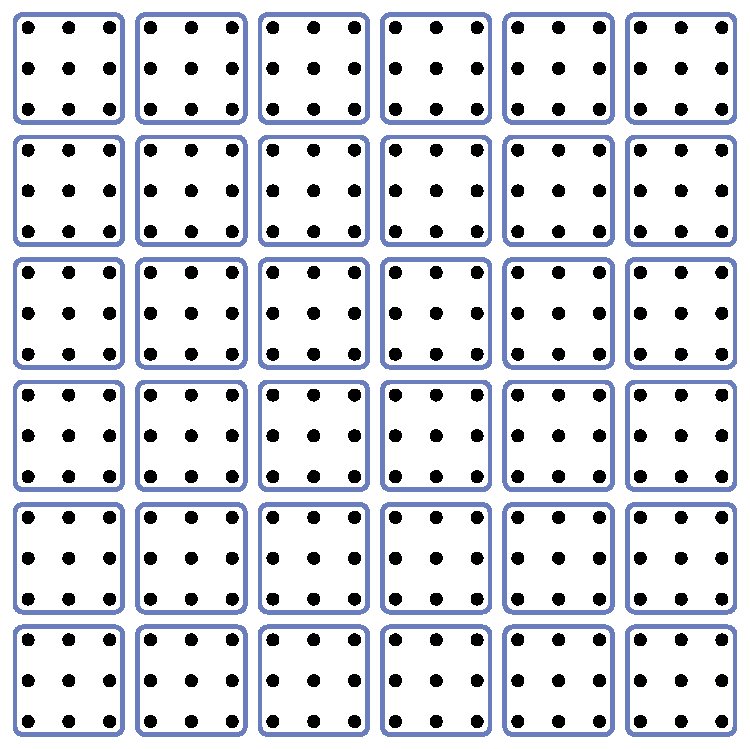
\includegraphics[width=.9\linewidth]{img/chap2/renorm_step1.pdf}
	\caption{Block spin averaging.}
	\label{renorm_1}
\end{subfigure}%
\begin{subfigure}{.25\textwidth}
	\centering
	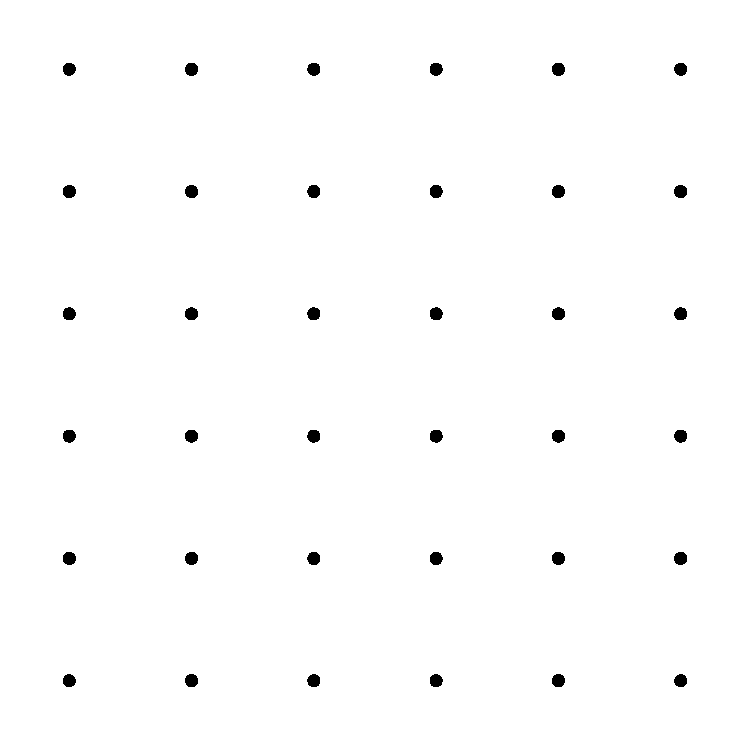
\includegraphics[width=.9\linewidth]{img/chap2/renorm_step2.pdf}
	\caption{The new lattice.}
	\label{renorm_2}
\end{subfigure}%
\begin{subfigure}{.25\textwidth}
	\centering
	
\includegraphics[width=.9\linewidth]{img/chap2/renorm_step3.pdf}
	\caption{Rescaling.}
	\label{renorm_3}
\end{subfigure}
\caption{The renormalization procedure illustrated. Here we have chosen $S = 3$.}
\label{fig:renorm_proc}
\end{figure}

Now we replace the microscopic Hamiltonian by an effective Hamiltonian for the block spin field $\tilde{\phi}$.
This Hamiltonian describe the new system depicted in fig. \eqref{renorm_2}. 
We are not done yet! To make the new system look as much as possible like the one we started from, we rescale all lengths (fig. \eqref{renorm_3}). We also rescale the field. Formally it means that we perform the change of variables
\begin{eqnarray}
x' = x/S  \\
\phi' = S^\Delta \tilde{\phi}
\end{eqnarray}
where $x$ could be any length appearing in the Hamiltonian.

The Hamiltonian in the new variables $H'[\phi'] = \tilde{H}[\tilde{\phi}]$ is the effective Hamiltonian after the renormalization operation.  
It could seem strange that we had to rescale the field as well as the lengths. We do that in order for the new Hamiltonian to resemble the old one as closely as possible. We are going to see on the example of the Lifshitz mean field theory how we can choose $\Delta$ for that purpose.

To conclude, the key ideas of the renormalization procedure are the averaging over block spins, and the rescaling of lengths and fields. We have described here the case of a discrete Hamiltonian, because it seemed more intuitive. But of course the ideas of renormalization are general and can as easily be applied to a continuous Hamiltonians.

\subsection{The renormalization group}

The Hamiltonian after the renormalization procedures writes
\begin{equation}
H'[\phi'] = \sum_{i'} \sum_\alpha \kappa_\alpha' O_\alpha[\phi'(i'), \nabla' \phi'(i'), ...]
\end{equation}
Couplings $\kappa$ are sent to new couplings $\kappa'$\footnote{It may also be that new couplings -- even infinitely many of them! -- are generated by the renormalization procedure. In that case, the structure of the Hamiltonian is not stable under renormalization, unless we already take into account these couplings at the microscopic scale, or unless we neglect them, thus making the renormalization procedure approximate.}, therefore we can define a \textit{group action} $g$, transforming the coupling constants at scale $1$ in the coupling constants at scale $S$:
\begin{equation}
\label{eq:rg_tranf}
\kappa_\alpha \rightarrow \kappa_\alpha' \define g(\kappa_\alpha, S)
\end{equation}
The renormalization group is a multiplicative, one parameter group:
\begin{equation}
g( g(\kappa_\alpha, S_1), S_2) = g(\kappa_\alpha, S_1 S_2)
\end{equation}
These transformations are assumed to be continuous in the coupling constants. It is also very often possible to consider the scale $S$ as a continuous parameter. Then the successive application of infinitesimally close renormalization group transformations generates a continuous trajectory in the space of coupling constants. This trajectory can be parametrized by $t \define \log(S)$, an additive parameter playing the role of a time. It is often referred to as ``the renormalization group time''.

Near a phase transition or critical point, fluctuations occur at all length scales, and thus one should expect the Hamiltonian to be scale invariant. 
In terms of the renormalization group action, scale invariance simply means that
\begin{equation}
g(\kappa_\alpha, S) = \kappa_\alpha
\end{equation}
The fact that scale invariance has such a simple meaning in the renormalization group framework is an extremely good sign. It is a hint that renormalization group is a powerful tool to look for critical points.

As an application of these ideas, imagine that we are close to a critical point. Then eq. \eqref{eq:rg_tranf} can be linearized:
\begin{equation}
\frac{d \log g(\kappa_\alpha, S)}{d \log S} = \lambda_\alpha
\end{equation}
If $\lambda_\alpha$ is positive, then the fixed point is repulsive in direction $\alpha$, and the coupling is said to be \textit{relevant}. On the other hand if $\lambda_\alpha$ is negative, the fixed point is attractive in this direction and the coupling is \textit{irrelevant}.

Let us imagine that we are at a point $g_0$ in the space of coupling constants, very close to a fixed point. If we do a small change in scale, taking us from $g_0$ to $g(S)$, then, because we are close to a fixed point, we have moved at first order in the direction of the most relevant coupling, let us say it is direction $\alpha = 0$. Then we have $ g(S) = g_0 S^{\lambda_0}$.
Under the same infinitesimal change in scale, the correlation length $\xi$ is transformed according to $\xi_{g_0} = S \xi_{g(S)} \propto S^{-1/\lambda}$. Usually, and also in the case of the Lifshitz model, the most relevant direction is that of temperature. Then the $\nu$ critical exponent is given by $\xi_{g_0} \propto |T - T_c|^{-\nu}$. 
By simple comparison with our result from the renormalization group, we have thus obtained the very important result
\begin{equation}
\nu = \frac{1}{\lambda_0}
\end{equation}
relating $\nu$, the critical exponent of the correlation length, to $\lambda_0$, the most relevant direction around a given fixed point.

\subsection{Renormalization procedure applied to the mean field Lifshitz theory}

As we have just seen, an operation from the renormalization group transforms our microscopic Hamiltonian $H$ into an effective Hamiltonian at scale $S$, $H_{S}$. 
Since our Hamiltonian is not isotropic (it distinguishes between the direction of the modulation $\sslash$, and the orthogonal direction $\perp$), we expect an operation of the renormalization group to change lengthscales by two different amounts in the two unequivalent directions. 
Scales in the parallel direction will be changed by a factor $S_\sslash$: $x_\sslash' = (S_\sslash)^{-1} x_\sslash$, while scales on the orthogonal direction will be changed by a factor $S_\perp$: $x_\perp' = (S_\perp)^{-1} x_\perp$.

To simplify things we can keep a single scale $S = S_\perp$, and define $\theta$ such that $S_\sslash = S^\theta$. Note that this is equivalent to changing the \textit{units} in the parallel direction: if we say that lengths in the orthogonal direction are measured in meters, then lengths in the parallel direction are measured in $(\text{meters})^\theta$.
A volume, which is normally measured in $(\text{meters})^d$ will in our new units system be measured in $(\text{meters})^{(d-m) + \theta m}$. It is as if $d$ had been replaced by
\begin{equation}
d_m \define d+ m(\theta -1)
\end{equation}

We define two anomalous dimensions by
\begin{align}
\langle \phi(p_\sslash) \phi(0) \rangle_{g^*} \propto |p_\sslash|^{\eta_\sslash -4} \\
\langle \phi(p_\perp) \phi(0) \rangle_{g^*} \propto |p_\perp|^{\eta_\perp -2} 
\end{align}
where $g^*$ is a fixed point in the space of coupling constants, and the proportionality constant is independent of the scale.

But we also know that
\begin{align}
\langle \phi(p_\sslash) \phi(0) \rangle_{g^*} \propto |p_\sslash|^{\frac{2 \Delta}{\theta}} \\
\langle \phi(p_\perp) \phi(0) \rangle_{g^*} \propto |p_\perp|^{2\Delta} 
\end{align}
where $\Delta$ is the renormalization of the field. 
Identifying these expressions for the renormalization of the correlation function with the previous ones, we can express $\Delta$ in two unequivalent ways, thus yielding an important relation between $\eta_\sslash$ and $\eta_\perp$:
\begin{equation}
\theta = \frac{2- \eta_\perp}{4- \eta_\sslash}
\end{equation}

\subsubsection{Mean field analysis}

We recall that the Lifshitz Hamiltonian is
\begin{equation}
H = \int_x \left( \frac{1}{2}(\partial_\perp \phi)^2 + \frac{\rho_0}{2} (\partial_\sslash \phi)^2 + \frac{\sigma_0}{2} (\partial_\sslash^2 \phi)^2 + U(\rho) \right)
\end{equation}

The mean field approximation consists in neglecting the fluctuations of the field. Therefore, the integration over the fluctuations performed during a renormalization group operation is trivial, and we can directly write the transformed Hamiltonian after a renormalization group operation $g(S)$ :
\begin{equation}
H'[\phi'] = \int_{x'} S^{d_m} \left( S^{-2\Delta -2} \frac{1}{2}(\partial_\perp' \phi')^2 + S^{-2\Delta -2 \theta} \frac{\rho_0}{2}  (\partial_\sslash' \phi')^2 + S^{-2\Delta - 4 \theta} \frac{\sigma_0}{2}  (\partial_\sslash'^2 \phi)^2 + U'(\phi') \right)
\end{equation}
This Hamiltonian must identify with the previous one, and in particular we must have $S^{d_m-2\Delta -2} =1$. This determines  the renormalization of the field at the mean field level.

As we have seen -- at least qualitatively, stripped pattern appear because of a nontrivial Laplacian squared term. Therefore at the Lifshitz point $\sigma_0$ must be nontrivial, and in particular must not renormalize away, which is only possible if $S^{d_m -2\Delta - 4 \theta} = 1$, \textit{i.e.} if
\begin{equation}
\theta =  \theta_{\text{mean field}}=  \frac{1}{2}
\end{equation}

In the mean field approximation, it is as if the physical dimension were
\begin{equation}
d_{\text{mean field}} = d - \frac{m}{2}
\end{equation}
We immediately deduce that the upper critical dimension\footnote{The upper critical dimension is the dimension above which mean field theory is exact, in the sense that it gives the correct critical exponents.}, which is ``normally'' 4, becomes
\begin{equation}
d_c^> = 4 + \frac{m}{2}
\end{equation}
around the Lifschitz point.

In real life materials, the most commonly encountered case is $m=1$ (when in the modulated phase, the field is periodic in one direction of space). In that case the upper critical dimension is $d_c^> = 4.5$. This is of course greater than $3$, so the critical exponents furnished by mean field analysis are incorrect in our tridimensional world! To have a better approximation of the critical exponents, we turn to the renormalization group tools.

\section{The nonperturbative renormalization group}

The idea of the nonperturbative renormalization group is to find an exact evolution equation of a scale-dependent object, which could possibly be the microscopic Hamiltonian, or the free energy, or the Legendre transform of the free energy: the effective action. 

We shall discuss here the so-called Wetterich equation \cite{Wetterich}, whose object of study is the scale dependent \textit{effective action} at scale $k$,  $\Gamma_k$. The effective action $\Gamma$ takes into account fluctuations on all length scales (\textit{i.e.} on all momentum scales), while $\Gamma_k$ only takes into account fluctuations of momentum (\textit{i.e.} inverse length scale) between $k$ and $\Lambda$.

\subsection{The scale-dependent effective action}

\begin{figure}[htp]
\begin{center}
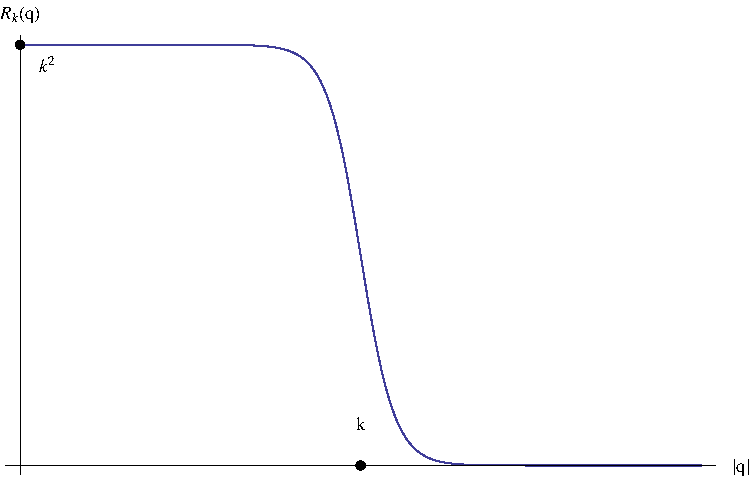
\includegraphics[scale=0.7]{img/chap2/regulator.pdf}
\caption{Typical shape of the regulator function in momentum space $R_k(q)$.}
\label{fig:regulator}
\end{center}
\end{figure}

Let us build $\Gamma_k$ explicitly.  To this end let us define the \textit{regulator} $R_k(x,y) = R(x) \delta(x-y)$, whose role is to give a mass to the modes of momentum smaller than $k$, while leaving the other modes untouched.
The typical shape of the regulator in momentum space is given by fig. \eqref{fig:regulator}. Moreover, the regulator is required to vanish at $k \rightarrow 0$ and to diverge for $k \rightarrow \infty$ (or $k \rightarrow \Lambda$), at fixed $q^2$. This can for example be achieved by
\begin{equation}
R_k(q) = \frac{q^2}{e^{q^2/k^2} - 1}
\end{equation}

We now introduce a modified, scale dependent Hamiltonian:
\begin{equation}
H_k[\varphi] \define H[\varphi] + \Delta H_k[\varphi], \text{~with~} \Delta H_k[\varphi] \define \frac{1}{2} \varphi \cdot R_k \cdot \varphi = \frac{1}{2} \int_{x,y} \varphi(x) R_k(x,y) \varphi(y)
\end{equation}

We see that the $\Delta H_k$ term is a quadratic on the field. Thus $R_k$ indeed acts as a scale-dependent and momentum-dependent squared mass term, giving a mass of order $k^2$ to the ``slow'' modes of momentum smaller than $k$.

We can now define the Legendre transform of the scale dependent free energy,
\begin{equation}
\label{eq:gamleg}
\gamleg[\phi] \define - W_k[h] + h \cdot \phi
\end{equation}
where the free energy is defined as $W_k[h] = \log Z_k$, and $Z_k = \int \D \varphi e^{-H_k[\varphi] + h \cdot \varphi} $.
Qualitatively, since the slow modes are given a mass in $W_k$, the Legendre transform only acts on the rapid modes, and we understand that  $\gamleg[\phi]$ indeed has the property of taking into accounts only rapid modes.\footnote{We note in passing that eq. \eqref{eq:gamleg} implies 
\begin{equation}
\phi(x) = \frac{\delta W_k[h]}{
\delta h(x)} = \frac{1}{Z_k[\varphi]} \int \D \varphi e^{-H_k[\varphi] + h \cdot \varphi} \varphi \define \langle \varphi(x) \rangle_k
\end{equation}
This tells us that $\phi$ is the background field (at scale $k$), \textit{i.e.} the mean value of the field $\varphi$ (at scale $k$). }

Finally, we introduce the scale-dependent effective action:
\begin{equation}
\gam_k[\phi] \define \gamleg[\phi] - \Delta H_k[\phi]
\end{equation}
This object has the right properties to be the effective action at scale $k$. Indeed it can be shown to verify $\gam_0 = \Gamma$, $\gam_\Lambda = H$.\footnote{The first identity is trivial, given the properties of the regulator function. Proving the second one requires slightly more work. It can be shown using that $\exp{-\Gamma_k[\phi]} = \int \D \varphi \exp{-S[\varphi] + \frac{\delta \Gamma}{\delta \varphi} \cdot (\varphi - \phi) - \frac{1}{2} (\varphi - \phi ) \cdot R_k \cdot (\varphi - \phi) }$, and remembering that $R_k \rightarrow \infty$ when $k \rightarrow \Lambda$.}


Finally, the scale-dependent effective action verifies the differential equation
\begin{equation}
\p{k} \gam_k[\phi] = \frac{1}{2} \int_{x,y} \p{k}\left(R_k(x,y)\right) \left( \Gamma^{(2)}_k(x,y) + R_k(x,y) \right)^{-1}
\end{equation}
This equation is often called the Wetterich equation. 
The demonstration can be found in appendix \eqref{app:wett}. We can use the fact that $R_k$ is invariant by translation, to write the right hand side of this integro-differential equation as a single integral over momentum $q$:
\begin{equation}
\p{k} \gam_k[\phi] = \frac{1}{2} \int_{q} \p{k}\left(R_k(q)\right) \left( \Gamma^{(2)}_k(q,-q) + R_k(q) \right)^{-1}
\end{equation}
Moreover, we shall make the change of variable $k \rightarrow t = \log(k/\Lambda)$, to take advantage of the additive properties of $t$\footnote{As we have seen before, $t$ can be regarded as a time parameterizing the renormalization group trajectory in the coupling constants space.}. In order to simplify further the Wetterich equation, we define an operator $\hat{\p{t}}$ as the differentiation with respect to $t$ acting only on $R_t$. That is,
\begin{equation}
 \hat{\p{t}} \define \frac{\partial R_t(\fdot)}{\partial t} \frac{\partial}{\partial R_t(\fdot)}
\end{equation}
where $R_t(\fdot)$ is a shorthand notation for the function $q \mapsto R_t(q)$. 
 We have then
\begin{equation}
\label{eq:wett}
\p{t} \gam_k[\phi] = \frac{1}{2} \hat{\p{t}} \tr{ \log\left( \Gamma^{(2)}_t(q,-q) + R_t(q) \right) }\footnote{Here we have used the formula for the trace on continuous indices in Fourier space: $\tr{A} = \int_{x} A(x,x) = \int_q A(q,-q)$.}
\end{equation}
This is the form of the Wetterich equation we will use from now on. 
Even if the field is vectorial, eq. \eqref{eq:wett} is still valid, provided that the trace acts on the vector space of the field as well\footnote{We refer to appendix \eqref{app:wett} for a sketch of proof.}.

Note that no approximations were made in the course of deriving the Wetterich equation. It is thus an exact equation describing the (renormalization group) time dependence of the scale-dependent effective action $\Gamma_t$, interpolating between $\Gamma_\Lambda = H$ and $ \Gamma_0 = \Gamma$.

We we can use the Wetterich equation as a starting point for finding the critical properties of the Lifshitz model.